% ============================================================
%  LaTeX CAPABILITIES SHOWCASE
%  A comprehensive sample document for university students
%  Demonstrating: typography, math, tables, figures, lists,
%  code listings, bibliography, cross-references, and more.
%
%  Author  : Farid Nahadi Muigu
%  Date    : March 2026
%  Compiler: pdfLaTeX  (run twice to resolve cross-references)
% ============================================================


% ────────────────────────────────────────────────────────────
%  DOCUMENT CLASS
%  'article'  – the most common class for papers / reports.
%  Other options: report, book, beamer (presentations)
%  [12pt]     – base font size
%  [a4paper]  – paper size
% ────────────────────────────────────────────────────────────
\documentclass[12pt, a4paper]{article}


% ════════════════════════════════════════════════════════════
%  PACKAGE IMPORTS
%  Packages extend LaTeX's core capabilities.
%  Each block below groups related packages together.
% ════════════════════════════════════════════════════════════

% --- ENCODING & LANGUAGE ----------------------------------------
\usepackage[T1]{fontenc}        % Proper font encoding (accents, etc.)
\usepackage[utf8]{inputenc}     % Accept UTF-8 source characters
\usepackage[english]{babel}     % Language-specific hyphenation & captions

% --- FONTS & TYPOGRAPHY -----------------------------------------
% mathpazo: Palatino for both text and math — warm, elegant, widely
% used in academic journals and textbooks (e.g., SIAM publications).
\usepackage{mathpazo}           % Palatino + Paleo math fonts
\usepackage{microtype}          % Micro-typographic enhancements (kerning, spacing)
\usepackage{setspace}           % Line-spacing control (\onehalfspacing etc.)
\usepackage{ragged2e}           % Better text alignment (RaggedRight etc.)
\onehalfspacing                 % Standard 1.5 line spacing

% --- PAGE LAYOUT ------------------------------------------------
\usepackage[
  top        = 2cm,
  bottom     = 2.5cm,
  left       = 1in,             % Binding margin
  right      = 1in,
  headheight = 15pt             % prevents fancyhdr headheight warning
]{geometry}                     % Full control over page margins

\usepackage{fancyhdr}           % Custom headers and footers
\usepackage{titlesec}           % Customize section heading styles
\usepackage{titling}            % Customize the \maketitle output
\usepackage{parskip}            % Space between paragraphs instead of indent
\usepackage{multicol}           % Multi-column layout

% --- COLORS & GRAPHICS ------------------------------------------
\usepackage[dvipsnames, svgnames, x11names]{xcolor}  % Named colours
\usepackage{graphicx}           % Include external images (\includegraphics)
\usepackage{tikz}               % Powerful in-document drawing
\usetikzlibrary{shapes.geometric, arrows.meta, positioning, shadows, patterns}
\usepackage{pgfplots}           % Bar charts and function plots (borrowed from UPRO template)
\pgfplotsset{compat=1.18}

% --- MATHEMATICS ------------------------------------------------
\usepackage{amsmath}            % Core math environments (align, equation, etc.)
\usepackage{amssymb}            % Extra math symbols (ℝ, ℕ, ∀, etc.)
\usepackage{amsthm}             % Theorem / Proof environments
\usepackage{mathtools}          % Extensions to amsmath (e.g. \coloneqq)
\usepackage{bm}                 % Bold math symbols (\bm{})

% --- TABLES -----------------------------------------------------
\usepackage{booktabs}           % Professional-quality horizontal rules in tables
\usepackage{array}              % Extended column types for tabular
\usepackage{multirow}           % Cells spanning multiple rows
\usepackage{tabularx}           % Auto-width columns (X type)
\usepackage{longtable}          % Tables that span multiple pages
\usepackage[table]{xcolor}      % Row/cell colouring in tables

% --- LISTS & ENUMERATIONS ---------------------------------------
\usepackage{enumitem}           % Fine-grained list customisation
\usepackage{mdwlist}            % Compact lists

% --- CODE LISTINGS ----------------------------------------------
\usepackage{listings}           % Source-code typesetting
\usepackage{lstautogobble}      % Auto-remove common leading whitespace

% --- CAPTIONS & FLOATS ------------------------------------------
\usepackage{caption}            % Customise figure/table captions
\usepackage{subcaption}         % Sub-figures and sub-tables
\usepackage{float}              % [H] placement specifier (Here, exactly)
\usepackage{wrapfig}            % Text wrapping around figures

% --- HYPERLINKS & PDF METADATA ----------------------------------
% NOTE: hyperref should almost always be the LAST package loaded.
\usepackage[hidelinks]{hyperref} % For hyperlinks

% --- BIBLIOGRAPHY -----------------------------------------------
\usepackage[round, authoryear, sort&compress]{natbib}
% natbib options: round brackets, author-year citations, sorted & compressed.
% If you prefer BibLaTeX with Biber instead:
%   \usepackage[backend=biber, style=authoryear, sorting=nyt]{biblatex}

% --- CALLOUT BOXES ----------------------------------------------
% tcolorbox lets us build professional alert/info/warning boxes that
% look like those in textbooks (Cambridge, MIT OpenCourseWare, etc.).
\usepackage[most]{tcolorbox}    % Rich coloured framed boxes

% --- MISCELLANEOUS ----------------------------------------------
\usepackage{lipsum}             % Generates placeholder (Lorem Ipsum) text
\usepackage{blindtext}          % Another placeholder-text generator
\usepackage{todonotes}          % Inline TODO notes during drafting
\usepackage{csquotes}           % Context-sensitive quotation marks


% ════════════════════════════════════════════════════════════
%  GLOBAL STYLE DEFINITIONS
%  Institutional aesthetic: restrained colour, clear hierarchy.
%  Inspiration: MIT OpenCourseWare, Cambridge lecture notes,
%  SIAM/Springer journal style guides.
% ════════════════════════════════════════════════════════════

% ── Colour palette: ONE primary accent + neutrals ──────────
% Institutional documents typically use a single accent colour,
% applied sparingly, with the rest being black / dark-grey.
\definecolor{InstBlue}{HTML}{1F3864}    % deep navy — dignified, serious
\definecolor{RuleGray}{HTML}{AAAAAA}    % subtle rule / border colour
\definecolor{LightGray}{HTML}{F7F7F7}   % very light table / box fill
\definecolor{DarkGray}{HTML}{444444}    % body-text softened black
\definecolor{CodeBg}{HTML}{F4F4F4}      % near-white code background
\definecolor{CodeKw}{HTML}{005B8E}      % muted code-keyword blue
\definecolor{CodeCmt}{HTML}{4A7C59}     % muted code-comment green
\definecolor{CodeStr}{HTML}{B03A2E}     % muted code-string red

% Backwards-compatible aliases: old colour names still appear in the
% document body (TikZ figures, tables) to demonstrate colour usage.
% We remap them to restrained institutional tones so the palette stays
% consistent without modifying every diagram.
\colorlet{PrimaryBlue}{InstBlue}           % navy (was bright cobalt)
\definecolor{AccentOrange}{HTML}{C0623A}   % muted terracotta (was vivid orange)
\definecolor{ForestGreen}{HTML}{3A6B45}    % earthier green

% ── Section heading styles — standard institutional style ───
% Plain bold numbering, consistent with most journals and textbooks.
% Each \section also starts on a fresh page (see etoolbox hook below).
\usepackage{etoolbox}            % pretocmd / apptocmd helpers

% Hyperlink Setup
\hypersetup{
    colorlinks=true,
    linkcolor=blue,
    filecolor=black,
    urlcolor=blue,
    citecolor=black,
    pdftitle={LaTeX Capabilities Showcase},
    pdfauthor={Farid Nahadi Muigu}
}

\titleformat{\section}
  {\normalfont\Large\bfseries}
  {\thesection}{1em}{}
\titlespacing*{\section}{0pt}{3.5ex plus 1ex minus .2ex}{2.3ex plus .2ex}

\titleformat{\subsection}
  {\normalfont\large\bfseries}
  {\thesubsection}{1em}{}
\titlespacing*{\subsection}{0pt}{3.25ex plus 1ex minus .2ex}{1.5ex plus .2ex}

\titleformat{\subsubsection}
  {\normalfont\normalsize\bfseries\itshape}
  {\thesubsubsection}{1em}{}

% ── Each section begins on its own page ────────────────────
% \pretocmd injects \clearpage before every \section call.
% \clearpage flushes all pending floats first, then starts a new page.
\pretocmd{\section}{\clearpage}{}{}

\urlstyle{same}

% ── Caption style (subtle, small, label in navy) ───────────
\captionsetup{
  font        = small,
  labelfont   = {bf, color=InstBlue},
  labelsep    = period,
  skip        = 6pt,
  format      = plain
}

% ── Code listing style (monochrome-friendly, print-safe) ───
\lstdefinestyle{mycodestyle}{
  backgroundcolor   = \color{CodeBg},
  basicstyle        = \ttfamily\small,
  keywordstyle      = \bfseries\color{CodeKw},
  commentstyle      = \itshape\color{CodeCmt},
  stringstyle       = \color{CodeStr},
  numberstyle       = \tiny\color{gray},
  numbers           = left,
  numbersep         = 10pt,
  stepnumber        = 1,
  showstringspaces  = false,
  breaklines        = true,
  breakatwhitespace = true,
  frame             = lines,          % top and bottom rules only (cleaner)
  framerule         = 0.5pt,
  rulecolor         = \color{RuleGray},
  xleftmargin       = 14pt,
  xrightmargin      = 4pt,
  aboveskip         = 10pt,
  belowskip         = 6pt,
  tabsize           = 2,
  autogobble        = true,
  captionpos        = b
}
\lstset{style=mycodestyle}

% ── tcolorbox callout environments ─────────────────────────
% These mimic the styled boxes in Cambridge/MIT lecture notes:
% a coloured left stripe, white interior, small bold header.
\tcbuselibrary{skins, breakable}

\newenvironment{notebox}[1][Note]{%
  \begin{tcolorbox}[
    enhanced, breakable,
    colback   = InstBlue!5,
    colframe  = InstBlue,
    leftrule  = 3.5pt, toprule=0.4pt, bottomrule=0.4pt, rightrule=0.4pt,
    arc       = 2pt,
    fonttitle = \bfseries\small,
    title     = #1,
    coltitle  = InstBlue,
    attach boxed title to top left = {yshift=-2mm, xshift=6pt},
    boxed title style = {colback=white, colframe=white, sharp corners}
  ]
}{\end{tcolorbox}}

\newenvironment{warningbox}[1][Warning]{%
  \begin{tcolorbox}[
    enhanced, breakable,
    colback   = black!4,
    colframe  = DarkGray,
    leftrule  = 3.5pt, toprule=0.4pt, bottomrule=0.4pt, rightrule=0.4pt,
    arc       = 2pt,
    fonttitle = \bfseries\small,
    title     = #1,
    coltitle  = DarkGray,
    attach boxed title to top left = {yshift=-2mm, xshift=6pt},
    boxed title style = {colback=white, colframe=white, sharp corners}
  ]
}{\end{tcolorbox}}

\newenvironment{tipbox}[1][Tip]{%
  \begin{tcolorbox}[
    enhanced, breakable,
    colback  = CodeCmt!8,
    colframe = CodeCmt,
    leftrule = 3.5pt, toprule=0.4pt, bottomrule=0.4pt, rightrule=0.4pt,
    arc      = 2pt,
    fonttitle = \bfseries\small,
    title    = #1,
    coltitle = CodeCmt!80!black,
    attach boxed title to top left = {yshift=-2mm, xshift=6pt},
    boxed title style = {colback=white, colframe=white, sharp corners}
  ]
}{\end{tcolorbox}}

% ── Page style — page number only, no header ───────────────
% \pagestyle{plain} would do this too, but using fancy gives us
% full control (e.g. if we later want to add a footer rule).
\pagestyle{fancy}
\fancyhf{}                          % clear ALL header and footer fields
\fancyfoot[C]{\small\thepage}       % centred page number in footer only
\renewcommand{\headrulewidth}{0pt}  % remove the header rule entirely
\renewcommand{\footrulewidth}{0pt}  % no footer rule either

% ── Theorem / Definition / Proof environments ──────────────
% amsthm lets us define custom theorem-like environments.
\theoremstyle{definition}
\newtheorem{definition}{Definition}[section]
\newtheorem{example}[definition]{Example}

\theoremstyle{plain}
\newtheorem{theorem}[definition]{Theorem}
\newtheorem{lemma}[definition]{Lemma}
\newtheorem{corollary}[definition]{Corollary}

\theoremstyle{remark}
\newtheorem*{remark}{Remark}

% ── Custom commands (macros) ────────────────────────────────
% Define frequently-used constructs as short commands:
\newcommand{\R}{\mathbb{R}}             % real numbers
\newcommand{\N}{\mathbb{N}}             % natural numbers
\newcommand{\Z}{\mathbb{Z}}             % integers
\newcommand{\C}{\mathbb{C}}             % complex numbers
\newcommand{\dx}{\,\mathrm{d}x}        % differential for integrals
\newcommand{\dt}{\,\mathrm{d}t}        % differential for integrals
\newcommand{\norm}[1]{\left\|#1\right\|}   % norm notation
\newcommand{\abs}[1]{\left|#1\right|}      % absolute value
\newcommand{\innerp}[2]{\langle #1,\, #2\rangle}  % inner product
\newcommand{\highlight}[1]{%
  \colorbox{InstBlue!12}{\textbf{#1}}}  % subtle highlighted key term
\newcommand{\email}[1]{\href{mailto:#1}{\texttt{#1}}}  % clickable email


% ════════════════════════════════════════════════════════════
%  DEDICATED COVER PAGE
%  Built manually (not via \maketitle) for full layout control.
%  Modelled after MIT OpenCourseWare / university lesson sheets.
% ════════════════════════════════════════════════════════════
% (Title is rendered inside \begin{document} — see below)


% ============================================================
%  BEGIN DOCUMENT
% ============================================================
\begin{document}

% ── Dedicated cover page ───────────────────────────────────
\begin{titlepage}
  \thispagestyle{empty}
  \centering
  \vspace*{2.5cm}

  % Institution / course block
  {\large\scshape Society of Marine Engieering Student\par}
  \vspace{0.3cm}
  {\normalsize In Collaboration With UNESCO JKUAT\par}
  \vspace{1.2cm}

  % Thick rule
  \noindent\rule{\linewidth}{0.8pt}
  \vspace{0.5cm}

  % Document type tag
  {\small \MakeUppercase{Lesson Handout}\par}
  \vspace{0.4cm}

  % Main title
  {\Huge \LaTeX{} Capabilities Showcase\par}
  \vspace{0.3cm}

  % Sub-title
  {\large\itshape A Comprehensive Reference for Students\par}
  \vspace{0.5cm}

  \noindent\rule{\linewidth}{0.8pt}
  \vspace{1.5cm}

  % Author block
  {\normalsize\textbf{Prepared by}\par}
  \vspace{0.3cm}
  {\large Farid Nahadi Muigu\par}
  {\normalsize\itshape nahadi.farid@students.jkuat.ac.ke\par}
  \vspace{1.5cm}


  \vfill

  \small This document is a comprehensive showcase of \LaTeX{}'s typesetting capabilities, intended for university students beginning to learn \LaTeX{}

\end{titlepage}

% ── Table of contents ──────────────────────────────────────
\tableofcontents
\listoffigures                  % list of all figures
\listoftables                   % list of all tables
\lstlistoflistings              % list of all code listings

\newpage                        % start content on a fresh page


% ============================================================
%  SECTION 1 – TEXT FORMATTING
% ============================================================
\section{Text Formatting}
\label{sec:text}

% ── 1.1 Basic text styles ──────────────────────────────────
\subsection{Basic Text Styles}

\LaTeX{} provides many ways to style text.  The most common are:

\begin{itemize}[
    leftmargin = 1.5em,
    itemsep    = 4pt,
    label      = \textcolor{AccentOrange}{\textbullet}]  % coloured bullets
  \item \textbf{Bold}: \verb|\textbf{text}|
  \item \textit{Italic}: \verb|\textit{text}|
  \item \texttt{Monospace}: \verb|\texttt{text}|
  \item \underline{Underline}: \verb|\underline{text}|
  \item \textsc{Small Caps}: \verb|\textsc{text}|
  \item \emph{Emphasis} (context-aware): \verb|\emph{text}|
  \item {\large Larger} or {\small Smaller} text via size declarations
  \item \textcolor{AccentOrange}{Coloured text} via \verb|\textcolor{colour}{text}|
\end{itemize}

% ── 1.2 Font sizes ─────────────────────────────────────────
\subsection{Font Size Hierarchy}

\LaTeX{} has a built-in size hierarchy (from smallest to largest):

\begin{center}
  {\tiny tiny} \quad
  {\scriptsize scriptsize} \quad
  {\footnotesize footnotesize} \quad
  {\small small} \quad
  {\normalsize normalsize} \quad
  {\large large} \quad
  {\Large Large} \quad
  {\LARGE LARGE} \quad
  {\huge huge} \quad
  {\Huge Huge}
\end{center}

% ── 1.3 Alignment ──────────────────────────────────────────
\subsection{Text Alignment}

\begin{flushleft}
  This paragraph is \textbf{left-aligned} (flushleft environment).
  \LaTeX{} normally justifies text to both margins, which is the typographic
  standard for books and academic papers.
\end{flushleft}

\begin{center}
  This paragraph is \textbf{centred} (center environment).
\end{center}

\begin{flushright}
  This paragraph is \textbf{right-aligned} (flushright environment).
\end{flushright}

% ── 1.4 Quotation environments ─────────────────────────────
\subsection{Quotations}

For a short inline quotation, use \texttt{\textbackslash enquote}:
\textit{``Typography is the art and technique of arranging type.''}

For a longer block quotation, use the \texttt{quote} environment:

\begin{quote}
  \textit{%
    ``Not everything that can be counted counts, and not everything that
    counts can be counted.''}\\
  \hfill --- William Bruce Cameron
\end{quote}

% ── 1.5 Footnotes ──────────────────────────────────────────
\subsection{Footnotes and Margin Notes}

Footnotes\footnote{This is a footnote. Use \texttt{\textbackslash footnote\{...\}}
to add one.} are easy in \LaTeX{}.  You can also add margin
notes\marginpar{\tiny Margin\\note here.} for editorial comments.

% ── 1.6 Line and page spacing ──────────────────────────────
\subsection{Spacing}

Horizontal space: A\hspace{1cm}B \quad (1 cm of explicit space between A and B).

Vertical space: use \verb|\vspace{0.5cm}| to add vertical gaps.

\vspace{0.4cm}

\noindent A horizontal rule spanning the full width:

\noindent\rule{\linewidth}{0.4pt}


% ============================================================
%  SECTION 2 – LISTS
% ============================================================
\section{Lists}
\label{sec:lists}

% ── 2.1 Unordered list ─────────────────────────────────────
\subsection{Unordered (Bullet) Lists}

\begin{itemize}
  \item First item
  \item Second item
    \begin{itemize}               % Nested list
      \item Nested item A
      \item Nested item B
        \begin{itemize}           % Doubly nested
          \item Deep item i
          \item Deep item ii
        \end{itemize}
    \end{itemize}
  \item Third item
\end{itemize}

% ── 2.2 Ordered list ───────────────────────────────────────
\subsection{Ordered (Numbered) Lists}

\begin{enumerate}[label=\textbf{\arabic*.}]  % enumitem: custom label format
  \item First step
  \item Second step
    \begin{enumerate}[label=\textbf{\alph*.}]
      \item Sub-step a
      \item Sub-step b
    \end{enumerate}
  \item Third step
\end{enumerate}

% ── 2.3 Description list ───────────────────────────────────
\subsection{Description Lists}

\begin{description}[style=nextline, leftmargin=2em]
  \item[\textcolor{PrimaryBlue}{pdfLaTeX}]
        Compiles \texttt{.tex} to PDF; supports most packages; the most
        widely-used engine.
  \item[\textcolor{PrimaryBlue}{XeLaTeX}]
        Supports Unicode and OpenType fonts natively; great for
        multi-lingual documents.
  \item[\textcolor{PrimaryBlue}{LuaLaTeX}]
        Like XeLaTeX but also allows embedded Lua scripting; very flexible.
\end{description}


% ============================================================
%  SECTION 3 – MATHEMATICS
% ============================================================
\section{Mathematics}
\label{sec:math}

Mathematics is arguably \LaTeX{}'s greatest strength.

% ── 3.1 Inline vs display ──────────────────────────────────
\subsection{Inline and Display Mode}

Inline maths is written between \verb|$...$|: the famous formula is
$e^{i\pi} + 1 = 0$ (Euler's identity).

Display (standalone) maths uses \verb|\[...\]| or the
\texttt{equation} environment:

% equation adds a number; equation* suppresses it.
\begin{equation}
  \label{eq:euler}
  e^{i\theta} = \cos\theta + i\sin\theta
\end{equation}

% ── 3.2 Fractions, roots, sums ─────────────────────────────
\subsection{Fractions, Roots, and Sums}

\[
  \sqrt[n]{a^n + b^n} \neq a + b
  \qquad
  \frac{\partial^2 u}{\partial t^2} = c^2 \nabla^2 u
  \qquad
  \sum_{k=0}^{\infty} \frac{(-1)^k}{2k+1} = \frac{\pi}{4}
\]

% ── 3.3 Integrals and limits ───────────────────────────────
\subsection{Integrals and Limits}

\[
  \int_{-\infty}^{+\infty} e^{-x^2} \dx = \sqrt{\pi}
  \qquad
  \lim_{x \to 0} \frac{\sin x}{x} = 1
  \qquad
  \oint_{\mathcal{C}} \mathbf{F} \cdot \mathrm{d}\mathbf{r} = 0
\]

% ── 3.4 Multi-line aligned equations ───────────────────────
\subsection{Aligned Equations}

The \texttt{align} environment aligns equations at the \texttt{\&} symbol:

\begin{align}
  (a + b)^2 &= a^2 + 2ab + b^2 \label{eq:square}\\
  (a - b)^2 &= a^2 - 2ab + b^2 \label{eq:diffsquare}\\
  (a + b)(a - b) &= a^2 - b^2   \label{eq:diffofquares}
\end{align}

We can reference numbered equations: Equation~\eqref{eq:euler} is Euler's
formula; Equation~\eqref{eq:square} expands a perfect square.

% ── 3.5 Matrices ───────────────────────────────────────────
\subsection{Matrices}

\[
  A = \begin{pmatrix}           % pmatrix → round brackets
    a_{11} & a_{12} & a_{13} \\
    a_{21} & a_{22} & a_{23} \\
    a_{31} & a_{32} & a_{33}
  \end{pmatrix},
  \qquad
  B = \begin{bmatrix}           % bmatrix → square brackets
    1 & 0 \\
    0 & 1
  \end{bmatrix}
\]

The determinant:
\[
  \det(A) = \begin{vmatrix}     % vmatrix → vertical bars
    a & b \\ c & d
  \end{vmatrix} = ad - bc
\]

% ── 3.6 Theorems, definitions, proofs ──────────────────────
\subsection{Theorems, Definitions, and Proofs}

\begin{definition}
  A function $f: \R^n \to \R$ is \textbf{convex} if for every
  $x, y \in \R^n$ and every $\lambda \in [0,1]$:
  \[
    f\bigl(\lambda x + (1-\lambda)y\bigr)
    \;\leq\;
    \lambda f(x) + (1-\lambda)f(y).
  \]
\end{definition}

\begin{theorem}[Cauchy–Schwarz Inequality]
  For all vectors $\mathbf{u}, \mathbf{v} \in \R^n$:
  \[
    \bigl|\innerp{\mathbf{u}}{\mathbf{v}}\bigr|^2
    \;\leq\;
    \innerp{\mathbf{u}}{\mathbf{u}} \cdot \innerp{\mathbf{v}}{\mathbf{v}}.
  \]
\end{theorem}

\begin{proof}
  Consider the function $f(t) = \norm{\mathbf{u} + t\mathbf{v}}^2 \geq 0$
  for all $t \in \R$.  Expanding and requiring the discriminant to be
  non-positive yields the result. \qed
\end{proof}

\begin{remark}
  Equality holds if and only if $\mathbf{u}$ and $\mathbf{v}$ are linearly
  dependent.
\end{remark}

% ── 3.7 Special sets and operators ─────────────────────────
\subsection{Special Symbols and Operators}

The standard number sets defined by our custom macros:
$\N \subset \Z \subset \R \subset \C$.

Greek letters appear frequently in mathematics:
$\alpha, \beta, \gamma, \delta, \epsilon, \zeta, \eta, \theta,
 \lambda, \mu, \xi, \pi, \rho, \sigma, \tau, \phi, \chi, \psi, \omega$.

Common operators: $\forall,\ \exists,\ \in,\ \notin,\ \subset,\ \cup,\
\cap,\ \oplus,\ \otimes,\ \nabla,\ \partial,\ \infty,\ \pm,\ \mp,\ \times,\
\div,\ \leq,\ \geq,\ \neq,\ \approx,\ \sim,\ \equiv,\ \propto$.

% ── 3.8 Cases and piecewise functions ──────────────────────
\subsection{Piecewise Functions}

\[
  |x| = \begin{cases}
           x  & \text{if } x \geq 0, \\
          -x  & \text{if } x < 0.
         \end{cases}
\]


% ============================================================
%  SECTION 4 – TABLES
% ============================================================
\section{Tables}
\label{sec:tables}

% ── 4.1 Basic booktabs table ───────────────────────────────
\subsection{Professional Table with Booktabs}

The \texttt{booktabs} package removes vertical lines and uses horizontal
rules to produce publication-quality tables (see Table~\ref{tab:basic}).

\begin{table}[H]
  \centering
  \caption{Comparison of common \LaTeX{} engines}
  \label{tab:basic}
  \begin{tabular}{llcc}
    \toprule
    \textbf{Engine}   & \textbf{Font Support} & \textbf{Unicode} & \textbf{Speed} \\
    \midrule
    pdfLaTeX          & Type-1, OTF (limited) & No               & Fast           \\
    XeLaTeX           & All OpenType          & Yes              & Moderate       \\
    LuaLaTeX          & All OpenType          & Yes              & Slower         \\
    \bottomrule
  \end{tabular}
\end{table}

% ── 4.2 Coloured table with multirow ───────────────────────
\subsection{Coloured Table with Multirow Cells}

Table~\ref{tab:coloured} demonstrates row colours and merged cells.

\begin{table}[H]
  \centering
  \caption{Grade distribution (sample data)}
  \label{tab:coloured}
  \rowcolors{2}{LightGray}{white}    % alternate row colours starting at row 2
  \begin{tabular}{lcc}
    \toprule
    \rowcolor{PrimaryBlue!20}
    \textbf{Grade Range} & \textbf{Letter} & \textbf{GPA Points} \\
    \midrule
    90 – 100             & A+              & 4.0                 \\
    80 – 89              & A               & 3.7                 \\
    70 – 79              & B               & 3.0                 \\
    60 – 69              & C               & 2.0                 \\
    50 – 59              & D               & 1.0                 \\
    \textless 50         & F               & 0.0                 \\
    \bottomrule
  \end{tabular}
\end{table}

% ── 4.3 tabularx (auto-width) ──────────────────────────────
\subsection{Auto-Width Columns with \texttt{tabularx}}

\begin{table}[H]
  \centering
  \caption{Common \LaTeX{} environments and their purposes}
  \label{tab:tabularx}
  \begin{tabularx}{\textwidth}{lX}          % X column fills remaining width
    \toprule
    \textbf{Environment}   & \textbf{Purpose}                             \\
    \midrule
    \texttt{equation}      & Display a single numbered mathematical expression.     \\
    \texttt{align}         & Align multi-line equations at a specific character.    \\
    \texttt{itemize}       & Create unordered (bulleted) lists.                     \\
    \texttt{enumerate}     & Create ordered (numbered) lists.                       \\
    \texttt{tabular}       & Construct tables with rows and columns (tabularx for auto-width X-columns). \\
    \texttt{figure}        & Float a figure (image or TikZ drawing) on the page.   \\
    \texttt{lstlisting}    & Display formatted source code.                         \\
    \texttt{theorem}       & State a mathematical theorem.                          \\
    \bottomrule
  \end{tabularx}
\end{table}


% ============================================================
%  SECTION 5 – FIGURES AND GRAPHICS
% ============================================================
\section{Figures and Graphics}
\label{sec:figures}

% ── 5.1 Including external images ──────────────────────────
\subsection{Including External Images}

Use \verb|\includegraphics| to embed images.  Supported formats include
PNG, JPG, and PDF.  The \texttt{width} option scales the image:

\begin{figure}[H]
  \centering
  % Replace the path below with your own image file.
  % Example:  \includegraphics[width=0.6\textwidth]{images/photo.png}
  %
  % Since we have no external image here, we draw a placeholder rectangle:
  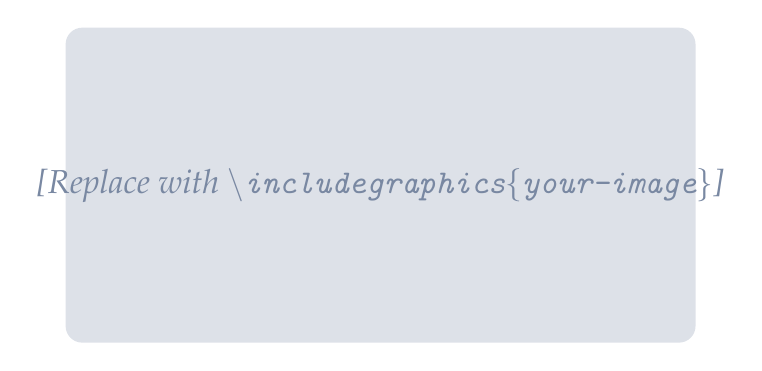
\begin{tikzpicture}
    \fill[PrimaryBlue!15, rounded corners=6pt] (0,0) rectangle (8,4);
    \node[text=PrimaryBlue!60, font=\large\itshape] at (4,2)
      {[Replace with \texttt{\textbackslash includegraphics\{your-image\}}]};
  \end{tikzpicture}
  \caption{A placeholder showing where an external image would appear.}
  \label{fig:placeholder}
\end{figure}

% ── 5.2 TikZ diagrams ──────────────────────────────────────
\subsection{TikZ Diagrams}

TikZ is a powerful in-document vector graphics library.
Figure~\ref{fig:tikz-flowchart} shows a simple flowchart drawn entirely
in \LaTeX{}.

\begin{figure}[H]
  \centering
  % ── TikZ node styles ──
  \tikzset{
    startstop/.style = {
      rectangle, rounded corners=8pt, minimum width=3cm, minimum height=1cm,
      text centered, draw=PrimaryBlue, fill=PrimaryBlue!20,
      font=\bfseries\small, drop shadow
    },
    process/.style = {
      rectangle, minimum width=3cm, minimum height=1cm,
      text centered, draw=AccentOrange, fill=AccentOrange!15,
      font=\small, drop shadow
    },
    decision/.style = {
      diamond, aspect=2, minimum width=3.2cm, minimum height=1cm,
      text centered, draw=ForestGreen!70!black, fill=ForestGreen!15,
      font=\small, drop shadow
    },
    arrow/.style = {thick, -Stealth, color=DarkGray}
  }
  \begin{tikzpicture}[node distance=1.5cm]
    % Nodes
    \node (start)   [startstop]                       {Start};
    \node (input)   [process,   below=of start]       {Read Input};
    \node (decide)  [decision,  below=of input]       {Valid?};
    \node (process) [process,   below=of decide]      {Process Data};
    \node (output)  [process,   below=of process]     {Output Result};
    \node (stop)    [startstop, below=of output]      {Stop};
    \node (error)   [process,   right=2.5cm of decide]{Show Error};

    % Arrows
    \draw [arrow] (start)   -- (input);
    \draw [arrow] (input)   -- (decide);
    \draw [arrow] (decide)  -- node[right]{Yes}  (process);
    \draw [arrow] (process) -- (output);
    \draw [arrow] (output)  -- (stop);
    \draw [arrow] (decide)  -- node[above]{No}   (error);
    \draw [arrow] (error)   |- (input);          % loop back
  \end{tikzpicture}
  \caption{A flowchart drawn entirely with TikZ inside \LaTeX{}.}
  \label{fig:tikz-flowchart}
\end{figure}

% ── 5.3 TikZ: function plot ────────────────────────────────
\subsection{Function Plot with TikZ}

\usetikzlibrary{calc}             % for coordinate calculations

\begin{figure}[H]
  \centering
  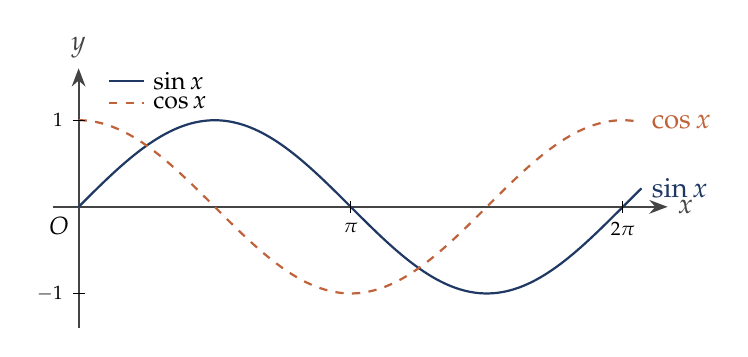
\begin{tikzpicture}[scale=1.1]
    % Draw axes
    \draw[-Stealth, thick, color=DarkGray] (-0.3,0) -- (6.8,0)
      node[right] {$x$};
    \draw[-Stealth, thick, color=DarkGray] (0,-1.4) -- (0,1.6)
      node[above] {$y$};

    % Plot sin(x) in blue
    \draw[thick, PrimaryBlue, domain=0:6.5, samples=200]
      plot (\x, {sin(\x r)})          % \x r = \x in radians
      node[right] {$\sin x$};

    % Plot cos(x) in orange (dashed)
    \draw[thick, AccentOrange, dashed, domain=0:6.5, samples=200]
      plot (\x, {cos(\x r)})
      node[right] {$\cos x$};

    % Origin label
    \node[below left, font=\small] at (0,0) {$O$};

    % x-axis ticks at multiples of π
    \foreach \k/\lab in {
        1/{$\pi$}, 2/{$2\pi$}}{
      \draw (\k*3.14159, 2pt) -- (\k*3.14159, -2pt)
        node[below, font=\scriptsize] {\lab};
    }

    % y-axis ticks
    \foreach \y in {-1, 1}{
      \draw (2pt, \y) -- (-2pt, \y)
        node[left, font=\scriptsize] {$\y$};
    }

    % Legend box
    \fill[white, opacity=0.8, rounded corners=3pt]
      (0.2, 1.1) rectangle (1.9, 1.55);
    \draw[thick, PrimaryBlue] (0.35,1.45) -- (0.75,1.45);
    \node[right, font=\small] at (0.75,1.45) {$\sin x$};
    \draw[thick, AccentOrange, dashed] (0.35,1.2) -- (0.75,1.2);
    \node[right, font=\small] at (0.75,1.2) {$\cos x$};
  \end{tikzpicture}
  \caption{Plots of $\sin x$ and $\cos x$ over $[0,\, 2\pi]$
           drawn with TikZ.}
  \label{fig:sincos}
\end{figure}

% ── 5.4 Sub-figures ────────────────────────────────────────
\subsection{Sub-Figures}

The \texttt{subcaption} package allows multiple figures side by side,
each with its own label (see Figure~\ref{fig:subfigs}).

\begin{figure}[H]
  \centering
  \begin{subfigure}[b]{0.45\textwidth}
    \centering
    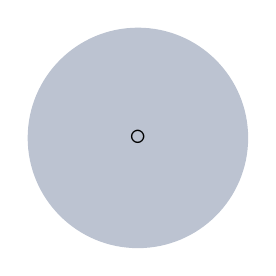
\begin{tikzpicture}
      \fill[PrimaryBlue!30] (0,0) circle (1.4cm);
      \node at (0,0) {\large$\circ$};
    \end{tikzpicture}
    \caption{A filled circle.}
    \label{fig:circle}
  \end{subfigure}
  \hfill
  \begin{subfigure}[b]{0.45\textwidth}
    \centering
    
\begin{tikzpicture}
      \fill[AccentOrange!40] (0,0) -- (2.8,0) -- (1.4,2.4) -- cycle;
    \end{tikzpicture}
    \caption{A filled triangle.}
    \label{fig:triangle}
  \end{subfigure}
  \caption{Two geometric shapes as sub-figures:
           (\subref{fig:circle}) circle and
           (\subref{fig:triangle}) triangle.}
  \label{fig:subfigs}
\end{figure}


% ============================================================
%  SECTION 6 – CODE LISTINGS
% ============================================================
\section{Code Listings}
\label{sec:code}

The \texttt{listings} package typesets source code with syntax colouring.

% ── 6.1 Python example ─────────────────────────────────────
\subsection{Python}

\begin{lstlisting}[language=Python, caption={Newton's method in Python.},
                   label={lst:python}]
  def newton(f, df, x0, tol=1e-9, max_iter=100):
      """
      Find a root of f using Newton-Raphson iteration.
      f   : function whose root is sought
      df  : derivative of f
      x0  : initial guess
      """
      x = x0
      for i in range(max_iter):
          fx = f(x)
          if abs(fx) < tol:
              return x, i        # (root approximation, iterations used)
          x -= fx / df(x)       # Newton update step
      raise RuntimeError("Did not converge after %d iterations." % max_iter)

  # Example usage: find sqrt(2) as root of f(x) = x^2 - 2
  import math
  root, n = newton(lambda x: x**2 - 2,
                   lambda x: 2*x,
                   x0=1.0)
  print(f"root = {root:.10f}  (exact: {math.sqrt(2):.10f})")
\end{lstlisting}

% ── 6.2 C example ──────────────────────────────────────────
\subsection{C}

\begin{lstlisting}[language=C, caption={Merge sort in C.}, label={lst:c}]
  #include <stdio.h>
  #include <stdlib.h>

  /* Merge two sorted sub-arrays of arr[]. */
  void merge(int *arr, int l, int m, int r) {
      int n1 = m - l + 1, n2 = r - m;
      int *L = malloc(n1 * sizeof(int));
      int *R = malloc(n2 * sizeof(int));
      for (int i = 0; i < n1; i++) L[i] = arr[l + i];
      for (int j = 0; j < n2; j++) R[j] = arr[m + 1 + j];
      int i = 0, j = 0, k = l;
      while (i < n1 && j < n2)
          arr[k++] = (L[i] <= R[j]) ? L[i++] : R[j++];
      while (i < n1) arr[k++] = L[i++];
      while (j < n2) arr[k++] = R[j++];
      free(L); free(R);
  }

  /* Recursive merge sort. */
  void mergeSort(int *arr, int l, int r) {
      if (l < r) {
          int m = l + (r - l) / 2;
          mergeSort(arr, l, m);
          mergeSort(arr, m + 1, r);
          merge(arr, l, m, r);
      }
  }
\end{lstlisting}

% ── 6.3 LaTeX snippet ──────────────────────────────────────
\subsection{\LaTeX{} Code Snippet}

\begin{lstlisting}[language={[LaTeX]TeX}, caption={A minimal \LaTeX{} document.},
                   label={lst:latexmin}]
  \documentclass[12pt, a4paper]{article}
  \usepackage{amsmath}

  \begin{document}
    \title{My First Document}
    \author{A University Student}
    \date{\today}
    \maketitle

    Hello, \LaTeX! The integral
    \[
      \int_0^\infty e^{-x^2}\,\mathrm{d}x = \frac{\sqrt{\pi}}{2}
    \]
    is the Gaussian integral.
  \end{document}
\end{lstlisting}


% ============================================================
%  SECTION 7 – CROSS-REFERENCING
% ============================================================
\section{Cross-Referencing}
\label{sec:xref}

\LaTeX{} provides a powerful labelling system.  Assign a label with
\verb|\label{key}| and reference it later with \verb|\ref{key}| or
\verb|\eqref{key}| (for equations) or \verb|\pageref{key}|.

\begin{itemize}
  \item Section~\ref{sec:math} (\textit{Mathematics}) is on
        page~\pageref{sec:math}.
  \item Euler's formula is Equation~\eqref{eq:euler}.
  \item The Cauchy–Schwarz table is Table~\ref{tab:basic}.
  \item The flowchart is Figure~\ref{fig:tikz-flowchart}.
  \item The Python listing is Listing~\ref{lst:python}.
\end{itemize}

The \texttt{hyperref} package (loaded in the preamble) automatically
converts all these references into \textbf{clickable hyperlinks} in the PDF.


% ============================================================
%  SECTION 8 – MULTI-COLUMN LAYOUT
% ============================================================
\section{Multi-Column Layout}
\label{sec:multicol}

The \texttt{multicol} package allows flowing text across several columns,
ideal for glossaries, indexes, or newspaper-style layouts.

\begin{multicols}{2}             % 2-column section
  \lipsum[1]                     % Lorem Ipsum placeholder text

  \columnbreak                   % force a column break

  \lipsum[2]
\end{multicols}


% ============================================================
%  SECTION 9 – SPECIAL ENVIRONMENTS
% ============================================================
\section{Special Environments}
\label{sec:special}

% ── 9.1 Callout boxes with tcolorbox ───────────────────────
\subsection{Information and Warning Boxes}

% The three environments below (notebox, warningbox, tipbox) are
% defined in the preamble using tcolorbox.  They mimic the styled
% callout boxes found in Cambridge and MIT Open­Course­Ware notes:
% a coloured left stripe, a bold title, and a lightly tinted interior.

\begin{notebox}[Note]
  Always compile a \LaTeX{} document \textbf{twice} (sometimes three
  times) so that cross-references and the table of contents are fully
  resolved.  The first pass writes label data; the second reads it.
\end{notebox}

\medskip

\begin{warningbox}[Warning]
  Never use the \texttt{eqnarray} environment --- it has subtle spacing
  bugs.  Use \texttt{align} (from \textsf{amsmath}) instead.  This is a
  well-known pitfall for \LaTeX{} beginners.
\end{warningbox}

\medskip

\begin{tipbox}[Tip]
  Use the \texttt{latexmk} command-line tool to automatically run
  \LaTeX{} the correct number of times, including BibTeX/Biber passes.
  Install it once: \texttt{sudo apt install latexmk}.
\end{tipbox}

% ── 9.2 Verbatim text ──────────────────────────────────────
\subsection{Verbatim Text}

The \texttt{verbatim} environment prints text \emph{exactly} as typed,
useful for showing command-line instructions:

\begin{verbatim}
    $ pdflatex sample_document.tex
    $ pdflatex sample_document.tex
    $ bibtex   sample_document
    $ pdflatex sample_document.tex
\end{verbatim}

For inline \verb|verbatim|, use: \verb|\verb|CODE||.

% ── 9.3 The todonotes package ──────────────────────────────
\subsection{\texttt{todonotes}: Draft Annotations}

During drafting, you can leave inline reminders:
%\todo{Replace this placeholder section with real content.}
% (The line above is commented out to keep the output clean.
%  Remove the leading % to activate it.)

The \verb|\todo{message}| command (from the \texttt{todonotes} package)
adds a coloured note in the margin and compiles a list of all TODOs.


% ============================================================
%  SECTION 10 – BIBLIOGRAPHY
% ============================================================
\section{Bibliography and Citations}
\label{sec:bib}

\LaTeX{} integrates tightly with BibTeX for managing references.

% ── 10.1 Citation commands ─────────────────────────────────
\subsection{Citation Styles}

The \texttt{natbib} package provides flexible citation styles:

\begin{itemize}
  \item Author-year: \texttt{\textbackslash citep\{knuth1984\}} →
        (Knuth, 1984)
  \item Textual: \texttt{\textbackslash citet\{lamport1994\}} →
        Lamport (1994)
  \item Numbered: with \verb|style=numeric| in \texttt{natbib}
\end{itemize}

The bibliography entries are stored in a \texttt{.bib} file (see the
\texttt{references.bib} file bundled with this sample).  Include them at
the end of the document with:

\begin{verbatim}
    \bibliographystyle{plainnat}
    \bibliography{references}
\end{verbatim}

% ── 10.2 Sample bibliography (in-line) ─────────────────────
\subsection{Sample \texttt{.bib} Entries}

A \texttt{.bib} file uses the following format:

\begin{lstlisting}[language={}, caption={Sample \texttt{.bib} entries.},
                   label={lst:bib}]
  @book{knuth1984,
    author    = {Donald E. Knuth},
    title     = {The {\TeX}book},
    publisher = {Addison-Wesley},
    year      = {1984}
  }

  @book{lamport1994,
    author    = {Leslie Lamport},
    title     = {{\LaTeX}: A Document Preparation System},
    publisher = {Addison-Wesley},
    edition   = {2nd},
    year      = {1994}
  }

  @article{einstein1905,
    author  = {Albert Einstein},
    title   = {{Zur Elektrodynamik bewegter K{\"o}rper}},
    journal = {Annalen der Physik},
    volume  = {322},
    number  = {10},
    pages   = {891--921},
    year    = {1905}
  }
\end{lstlisting}


% ============================================================
%  SECTION 11 – ADVANCED TYPOGRAPHY
% ============================================================
\section{Advanced Typography Tips}
\label{sec:typo}

\subsection{Dashes and Hyphens}

\LaTeX{} distinguishes three types of horizontal dashes:

\begin{center}
  \begin{tabular}{lll}
    \toprule
    \textbf{Name}  & \textbf{Source}    & \textbf{Result}  \\
    \midrule
    Hyphen         & \texttt{-}         & Self-reference   \\
    En dash        & \texttt{--}        & pages 10--20     \\
    Em dash        & \texttt{---}       & He paused---then spoke \\
    \bottomrule
  \end{tabular}
\end{center}

\subsection{Proper Quotation Marks}

In \LaTeX{}, \emph{never} use the keyboard double-quote character directly.
Instead:
\begin{itemize}
  \item Single quotes: \texttt{`text'} → `text'
  \item Double quotes: \texttt{``text''} → ``text''
\end{itemize}

\subsection{Non-Breaking Spaces and Fine Spacing}

Use a tilde \texttt{$\sim$} for a non-breaking space (e.g.\
\texttt{Figure$\sim$\textbackslash ref\{...\}}) so that the figure number
never wraps to the next line.

Use \verb|\,| for a thin space in formulae: $f\colon \R \to \R$
vs.\ $f: \R \to \R$.

\subsection{Microtype Enhancements}

The \texttt{microtype} package (loaded in the preamble) automatically
applies character protrusion and font expansion, making paragraphs look
more balanced with fewer hyphenation breaks — no user action required.


% ============================================================
%  SECTION 12 – DOCUMENT ORGANISATION TIPS
% ============================================================
\section{Organising Large Documents}
\label{sec:organisation}

\begin{description}[style=nextline, leftmargin=2.2em]
  \item[\texttt{\textbackslash input\{file\}}]
    Inserts \texttt{file.tex} inline — errors are reported with line
    numbers relative to the \emph{parent} file.
  \item[\texttt{\textbackslash include\{file\}}]
    Like \texttt{\textbackslash input} but adds a \texttt{\textbackslash clearpage}
    before/after and supports \texttt{\textbackslash includeonly\{\}} for
    selective compilation (faster when working on large manuscripts).
  \item[Class \texttt{report} / \texttt{book}]
    For multi-chapter documents use \texttt{report} (chapters, no recto/verso)
    or \texttt{book} (chapters, recto/verso layout, frontmatter/mainmatter/backmatter).
  \item[Version control]
    Store your \texttt{.tex} and \texttt{.bib} files in Git.  Add
    \texttt{*.aux}, \texttt{*.log}, \texttt{*.out}, \texttt{*.pdf} to
    \texttt{.gitignore}.
\end{description}

% ── Summary table: what each section covered ───────────────
\subsection{Quick Reference: What We Covered}

\begin{table}[H]
  \centering
  \caption{Summary of topics demonstrated in this document.}
  \label{tab:summary}
  \begin{tabularx}{\textwidth}{lX}
    \toprule
    \textbf{Topic}            & \textbf{Packages / Commands Used}                   \\
    \midrule
    Text formatting           & Core \LaTeX{}, \texttt{xcolor}, \texttt{setspace}   \\
    Lists                     & \texttt{enumitem}                                   \\
    Mathematics               & \texttt{amsmath}, \texttt{amssymb}, \texttt{amsthm},
                                \texttt{mathtools}                                   \\
    Tables                    & \texttt{booktabs}, \texttt{tabularx}, \texttt{multirow},
                                \texttt{xcolor} (rows)                               \\
    Figures / graphics        & \texttt{graphicx}, \texttt{tikz}, \texttt{subcaption}\\
    Code listings             & \texttt{listings}                                   \\
    Cross-referencing         & \texttt{hyperref}, \texttt{\textbackslash label}/\texttt{\textbackslash ref} \\
    Multi-column layout       & \texttt{multicol}                                   \\
    Info/warning boxes        & \texttt{tikz}                                       \\
    Bibliography              & \texttt{natbib}, BibTeX                             \\
    Typography                & \texttt{microtype}, \texttt{fontenc}, \texttt{babel} \\
    Large-doc organisation    & \verb|\input|/\verb|\include|, document classes      \\
    \bottomrule
  \end{tabularx}
\end{table}


% ============================================================
%  BACK MATTER
% ============================================================

% ── Appendix ───────────────────────────────────────────────
\appendix                        % \section now generates Appendix A, B, ...

\section{Useful \LaTeX{} Resources}
\label{app:resources}

\begin{itemize}
  \item \href{https://www.overleaf.com/learn}{Overleaf Documentation} —
        the most beginner-friendly online reference.
  \item \href{https://en.wikibooks.org/wiki/LaTeX}{\LaTeX{} Wikibook} —
        comprehensive free textbook.
  \item \href{https://ctan.org}{CTAN (Comprehensive TeX Archive Network)} —
        all \LaTeX{} packages and their documentation.
  \item \href{https://tex.stackexchange.com}{tex.stackexchange.com} —
        the best Q\&A community for \LaTeX{} questions.
  \item Donald E.\ Knuth, \textit{The \TeX{}book} (1984) — the definitive
        reference for the underlying \TeX{} engine.
  \item Leslie Lamport, \textit{\LaTeX{}: A Document Preparation System}
        (2nd ed., 1994) — the original \LaTeX{} manual.
\end{itemize}


% ── Bibliography ───────────────────────────────────────────
% Uncomment the two lines below once you have a references.bib file:
% \bibliographystyle{plainnat}
% \bibliography{references}

% ── End of document ────────────────────────────────────────
\end{document}
% ============================================================
%  END OF SAMPLE DOCUMENT
% ============================================================
